
\documentclass[12pt]{article}
\usepackage[brazil]{babel}
\usepackage[utf8]{inputenc}
\usepackage{amsmath}
\usepackage{amsfonts}
\usepackage{amssymb}
\usepackage{geometry}
\usepackage{graphicx}
\usepackage{float}
\usepackage{enumitem}
\usepackage{multicol}
\usepackage{array}
\usepackage{xcolor}
\usepackage[T1]{fontenc}
\usepackage{mathptmx} %times new roman


\geometry{a4paper, margin=1.2cm}
\setlength{\parindent}{0cm}

% implementa contador
% Definindo o contador e o comando de questão
\newcounter{questao}
\newcommand{\novaquestao}[1]{%
	\stepcounter{questao}%
	\subsection*{Questão \thequestao\ (#1)}%
}

\begin{document}
	\large
	\thispagestyle{empty}
	% Cabeçalho reduzido
	\vspace{0.5cm}
	\begin{center}
		\large
		\begin{tabular}{|l l|}
			\hline
			\textbf{ESCOLA:} & EETI GILBERTO MESTRINHO DE MEDEIROS RAPOSO \\ 
			\textbf{ALUNA(O):} & \underline{\hspace{7cm}} \textbf{SÉRIE:} \underline{\hspace{1.5cm}} \textbf{TURMA:} \underline{\hspace{1.5cm}} \\
			\textbf{PROFESSOR:} & \underline{\hspace{7cm}} \textbf{DATA:} \underline{\hspace{1.5cm}}/\underline{\hspace{1.5cm}}/\underline{\hspace{1.5cm}} \\
			\textbf{VALOR:} & \underline{\hspace{3cm}} \textbf{NOTA:} \underline{\hspace{1.5cm}} \\
			\hline
		\end{tabular}
	\end{center}
	\vspace{0.5cm}
	
	% Título manual
	\begin{center}
		\Large\textbf{AV1 - 3º BIMESTRE}
	\end{center}
	
	\vspace{0.3cm}
	
	\section*{\textbf{ATENÇÃO:}}
	\begin{itemize}[noitemsep]
		\item Resolva toda a PROVA, justificando cada questão.
		\item Colocar o nome completo e identificação no cabeçalho.
		\item Há apenas uma opção correta em cada questão de múltipla escolha.
	\end{itemize}
	% Início das colunas com linha vertical
	%\mostravermelhotrue
	\begin{multicols}{2}
		\columnseprule=0.4pt
		\columnsep=20pt
		
		\novaquestao{Enem 2023}
		
			No alojamento de uma universidade, há alguns quartos com o padrão superior ao dos demais. Um desses quartos ficou disponível, e muitos estudantes se candidataram para morar no local. Para escolher quem ficará com o quarto, um sorteio será realizado. Para esse sorteio, cartões individuais com os nomes de todos os estudantes inscritos serão depositados em uma urna, sendo que, para cada estudante de primeiro ano, será depositado um único cartão com seu nome; para cada estudante de segundo ano, dois cartões com seu nome; e, para cada estudante de terceiro ano, três cartões com seu nome. Foram inscritos 200 estudantes de primeiro ano, 150 de  segundo ano e 100 de terceiro ano. Todos os cartões têm a mesma probabilidade de serem sorteados. Qual a probabilidade de o vencedor do sorteio ser um estudante de terceiro ano?
		
			\begin{enumerate}[label=(\alph*), noitemsep]
				\item {1}/{2}
				\item {1}/{3}
				\item {1}/{8}
				\item {2}/{9}
				\item {3}/{8}
			\end{enumerate}
		
		\novaquestao{Enem 2019}
		
			Em um determinado ano, os computadores da receita federal de um país identificaram como inconsistentes 20\% das declarações de imposto de renda que lhe foram encaminhadas. Uma declaração é classificada como inconsistente quando apresenta algum tipo de erro ou conflito nas informações prestadas. Essas declarações 
			consideradas inconsistentes foram analisadas pelos auditores, que constataram que 25\% delas eram fraudulentas. Constatou-se ainda que, dentre as declarações que não apresentaram inconsistências, 6,25\% eram fraudulentas. Qual é a probabilidade de, nesse ano, a declaração de um contribuinte ser considerada inconsistente, dado 
			que ela era fraudulenta?
		
			\begin{enumerate}[label=(\alph*), noitemsep]
				\item 0,0500
				\item 0,1000
				\item 0,1125
				\item 0,3125
				\item 0,5000
			\end{enumerate}
		
		\novaquestao{UEA SIS II 2016}
		
			Em uma urna há 20 bolas numeradas de 20 a 39. Retirando-se aleatoriamente uma bola dessa urna, a probabilidade de que o número da bola seja múltiplo de 3 e que a soma dos algarismos seja menor ou igual a 7 é:
			
			\begin{enumerate}[label=(\alph*), noitemsep]
				\item {3}/{5}
				\item {2}/{5} 
				\item {1}/{5} %
				\item {3}/{20} 
				\item {1}/{20}
			\end{enumerate}
		
		\novaquestao{UEA SIS II 2012}
		
			Em um cesto há 250 camu-camus, dos quais 20\% estão verdes
			e 500 acerolas, das quais 15\% também estão verdes. Se uma pessoa
			retirar ao acaso um fruto desses cesto, a probabilidade de que o 
			fruto esteja verde é:
			
			\begin{enumerate}[label=(\alph*), noitemsep]
				\item {2}/{3}
				\item {1}/{3}
				\item {1}/{4}
				\item {1}/{5}  
				\item {1}/{6} %
			\end{enumerate}
		
		\novaquestao{UFU-MG 2018}
		
			As irmãs Ana e Beatriz e seus respectivos namorados vão sentar-se em um banco de 
			jardim (figura) de modo que cada namorado fique ao lado de sua namorada.
			
			\begin{center}
				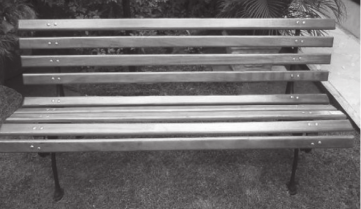
\includegraphics[scale=0.6]{imagens/ufu-2018.png}
			\end{center} A probabilidade de as irmãs sentarem-se uma ao lado da outra é igual a:
			
			\begin{enumerate}[label=(\alph*), noitemsep]
				\item 0,25
				\item 0,33
				\item 0,45
				\item 0,50
				\item 0,75
			\end{enumerate}
		
		\novaquestao{Enem 2020}

            Nos livros Harry Potter, um anagrama do nome do personagem “TOM MARVOLO RIDDLE” gerou a frase “I AM LORD VOLDEMORT”.
            
            Suponha que Harry quisesse formar todos os anagramas da frase “I AM POTTER”, de tal forma que as vogais e consoantes aparecessem sempre intercaladas, e sem considerar o espaçamento entre as letras.
            
            Nessas condições, o número de anagramas formados é dado por

                \begin{enumerate}[label=(\alph*) , noitemsep]
                \item $9!$.
                \item $4! \ 5!$.
                \item $2 \times 4! \ 5!$.
                \item $\frac{9!}{2!}$.
                \item $\frac{4! \ 5!}{2}$.
                \end{enumerate}
                        		
	\novaquestao{Enem 2019}

            Durante suas férias, oito amigos, dos quais dois são canhotos, decidem realizar um torneio de vôlei de praia. Eles precisam formar quatro duplas para a realização do torneio. Nenhuma dupla pode ser formada por dois jogadores canhotos.

            De quantas maneiras diferentes podem ser formadas
            essas quatro duplas?

                \begin{enumerate}[label=(\alph*), noitemsep]
                \item 69.
                \item 70.
                \item 90.
                \item 104.
                \item 105.
                \end{enumerate}

        \novaquestao{Enem 2012}

            O diretor de uma escola convidou os 280 alunos de terceiro ano a participarem de uma brincadeira. Suponha que existem 5 objetos e 6 personagens numa casa de 9 cômodos: um dos personagens esconde um dos objetos em um dos cômodos da casa. O objetivo da brincadeira é adivinhar qual objeto foi escondido por qual personagem e em qual cômodo da casa o objeto foi escondido.

            Todos os alunos decidiram participar. A cada vez um, aluno é sorteado e dá a sua resposta. As respostas devem ser sempre distintas das anteriores, e um mesmo aluno não pode ser sorteado mais de uma vez. Se a resposta do aluno estiver correta, ele é declarado vencedor e a brincadeira é encerrada.
            
            O diretor sabe que algum aluno acertará a resposta porque há

                \begin{enumerate}[label=(\alph*), noitemsep]
                \item 10 alunos a mais do que possíveis respostas distintas.
                \item 20 alunos a mais do que possiveis respostas distintas.
                \item 119 alunos a mais do que possiveis respostas distintas.
                \item 260 alunos a mais do que possíveis respostas distintas.
                \item 270 alunos a mais do que possíveis respostas distintas.
                \end{enumerate}


        \novaquestao{UEA 2009}

            Um determinado artesanato terá uma faixa colorida composta de três listas de cores distintas, uma lista abaixo da outra. As cores utilizadas serão azul, vermelha e laranja. O número de maneiras distintas em que essas listas coloridas podem ser dispostas de forma que as cores azul e vermelha fiquem sempre juntas é 

                \begin{enumerate}[label=(\alph*), noitemsep]
                \item 2.
                \item 4.
                \item 6.
                \item 8.
                \item 9.
                \end{enumerate}

        \novaquestao{UFAM 2020}

          As prateleiras de um determinado compartimento são identificadas por meio de números pares formados com 3 elementos do conjunto $C = \{2,3,4,6,7\}$. Nessas condições, é CORRETO afirmar que o número máximo de prateleiras desse compartimento é:

                \begin{enumerate}[label=(\alph*), noitemsep]
                \item 38.
                \item 42.
                \item 56.
                \item 60.
                \item 75.
                \end{enumerate}
		
		
		
	\end{multicols}
	
\end{document}
